\chapter{緒論}

\section{動機}

隨著遊戲的發展,現代的遊戲越來越趨於複雜,從數人的小型獨立製作,到數百人的大型 3A 級遊戲,遊戲的規模與以前不可同日而語,現今一個獨立開發工作室製作的 2D 遊戲,
在十多年前要達到同樣的規模可能要數十人的團隊才可能達到,而這些節省下來的時間成本,就是多虧了遊戲引擎的強大之處。現代遊戲引擎的複雜度,先進的圖學技術,複雜的物理模擬,
是需要一個具有規模的團隊來開發的,我們嘗試以此為目標,試著實作了一個具有一定規模的 2D 遊戲引擎。

\section{問題描述}

\subsection{歷史介紹}

最初並沒有所謂的遊戲引擎,遊戲常常是重頭開始建構(from scratch)的,這個概念被眾人所知最早是由 Jhon Carmack 發揚光大,他為 Doom 以及 Quake 系列遊戲開發的 3D 遊戲引擎,
深深地影響了遊戲業界,為早期(1990末)的遊戲業界標準,並促成引擎授權的商業模式,使得遊戲軟體的規模上升。

\subsection{遊戲是什麼}
電腦遊戲的技術本質是實時(real-time)可交互(interactive)的程式,遊戲程式會模擬出不精確但足以表現的遊戲世界,並且根據玩家的輸入做出相對的輸出(例如操作搖桿控制角色等),
通常遊戲會實作遊戲循環(Game Loop),更新遊戲邏輯、物理模擬、更新 AI 等。而通常遊戲要維持在每秒更新 60 幀才能保證流暢運行(低於 60 fps 通常會感覺卡頓),
也就是要在 16 毫秒內做完所有的遊戲更新並渲染到螢幕上頭,更何況在 VR 上要維持 90 FPS 才不會感覺暈眩,這也是為甚麼遊戲會如此要求效能。

\subsection{遊戲引擎是什麼}

遊戲引擎(Game Enigne)從字面上解釋是驅動遊戲的基礎程式,因此遊戲引擎須具備了窗口管理、輸出入管理、渲染(Rendering)系統、物理(Physics)系統…等子系統,除了基礎程式之外,
要是一個遊戲引擎還必須要有讓遊戲開發者使用之工具(可視化、非可視化),可能是單個工具或一整個工具鏈(Toolchain),使得遊戲開發者可以用該工具開發遊戲(Developing)、
進行測試(Debugging)、封裝發布(Shipping)等,否則就只能被稱為遊戲框架(Game Framework)。
遊戲引擎會讀入自訂的資源(Asset)格式 \footnote{常常是為了效能才會這樣做},並且有工具支援設計師將素材(貼圖、音效、模型等)轉換成引擎的格式,或是引擎工具可以直接產生,
因此遊戲引擎可以說是專門開發遊戲的開發環境。

\subsection{遊戲引擎具備的功能}

一個遊戲引擎要具備的功能非常多,並且功能以層層分開,上層依賴的下層的功能實現,從底層的硬體、作業系統,接著是使用的函式庫,接著核心系統例如:視窗函式庫、檔案系統、網路、序列化、型別資訊等。
再上層有資源管理(素材載入)、渲染器(Renderer)、物理引擎等子系統,可見遊戲引擎的龐大。 \cite{Gregory.2018}

\begin{figure}[h]
    \begin{center}
    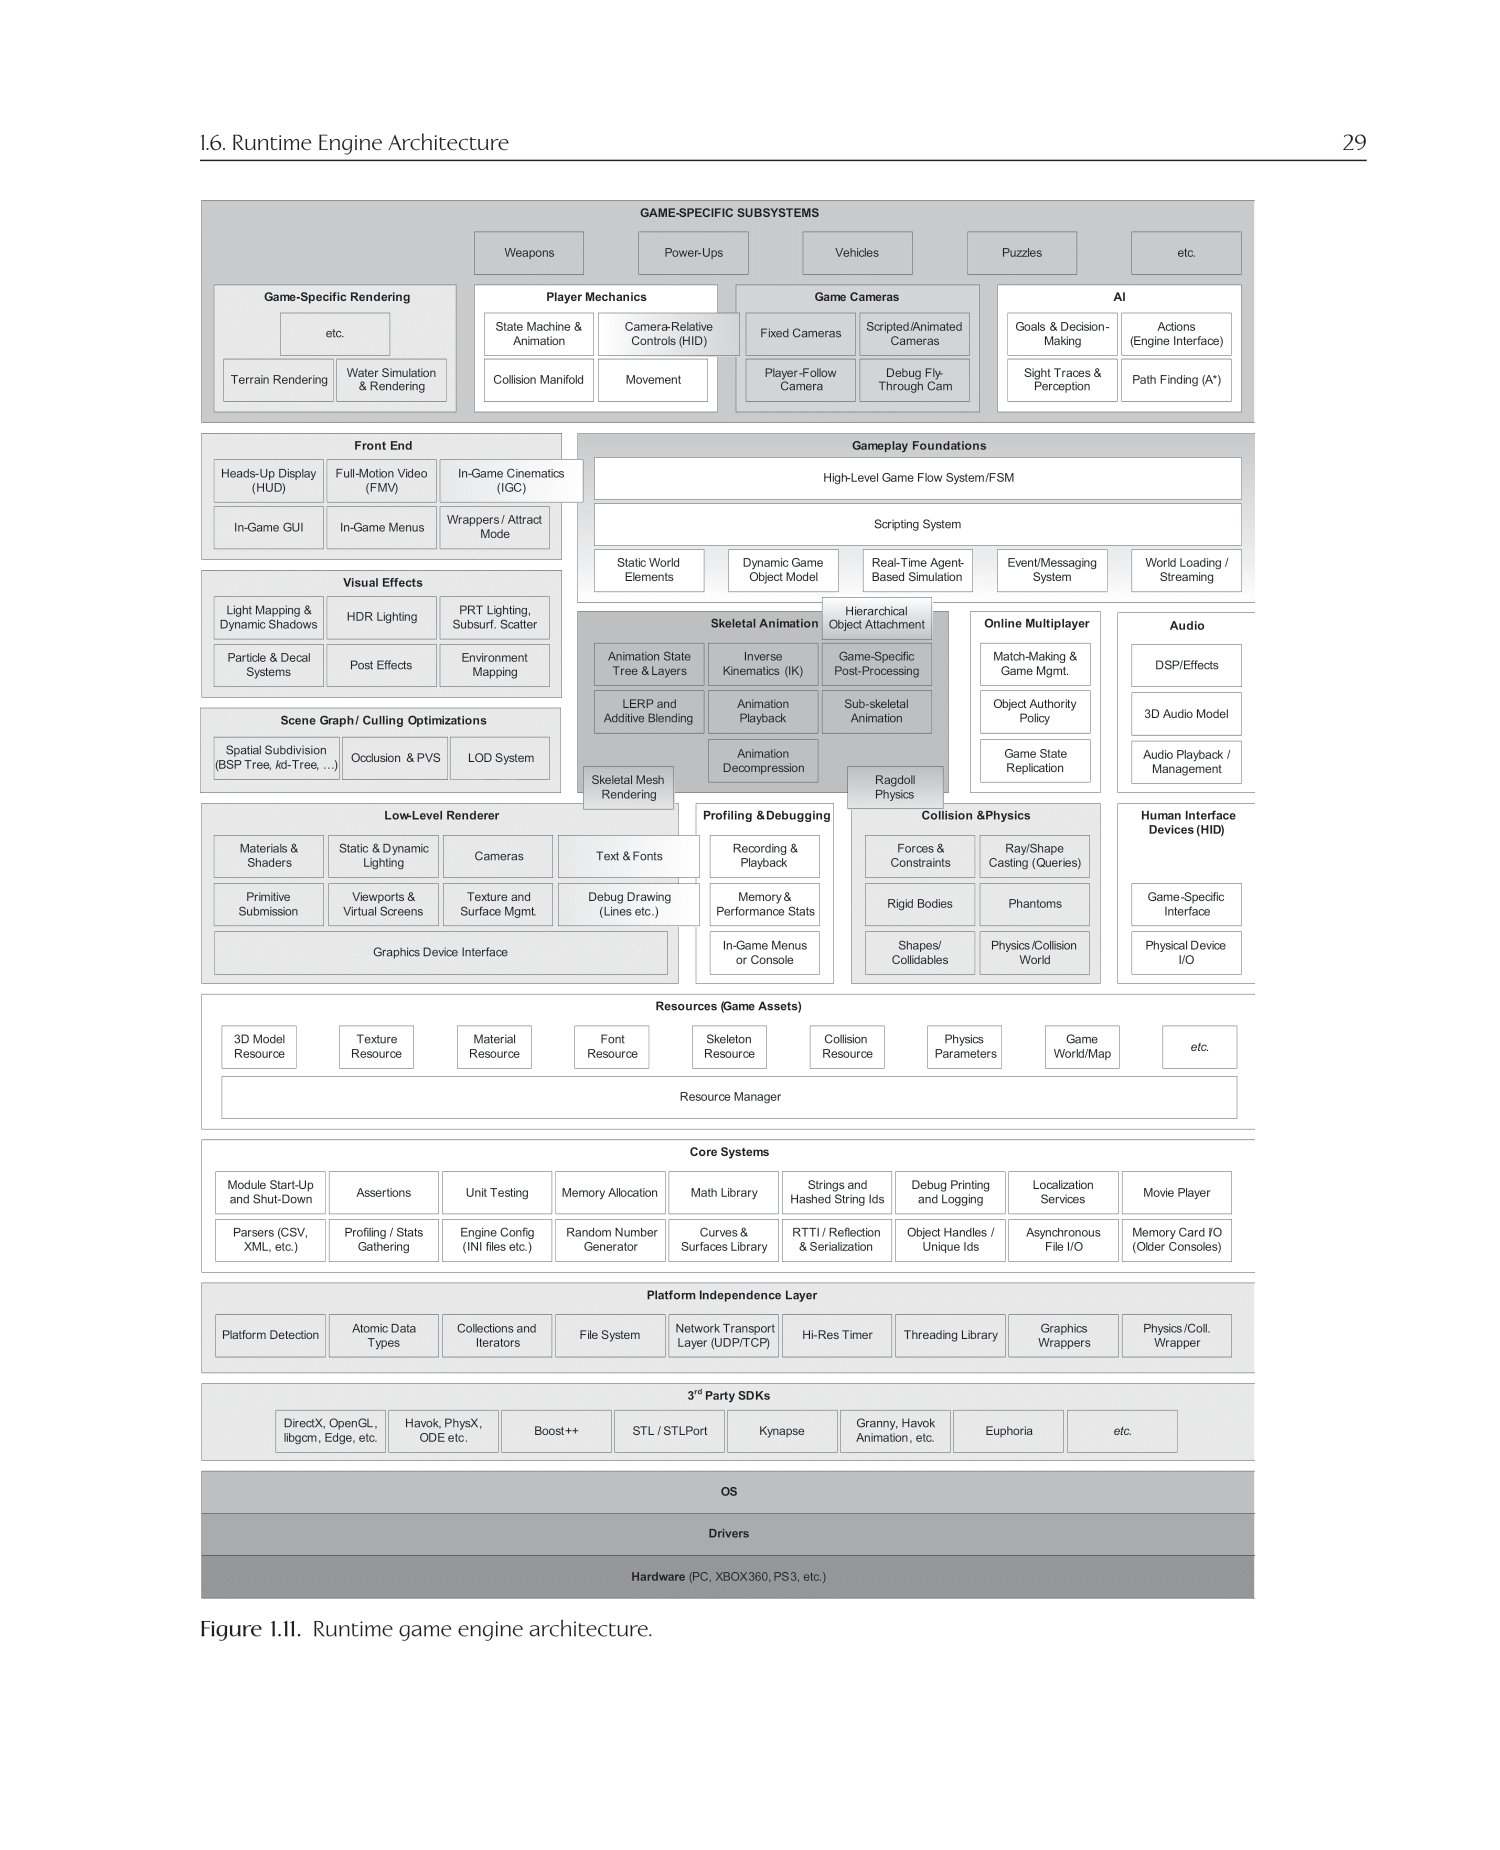
\includegraphics[width=\textwidth]{./resources/engine_arch.png}
    \end{center}
\caption{Game Engine Architecture}
\label{fig:EngineArch}
\end{figure}

\newpage